\documentclass[border=4pt]{standalone}
% Preámbulo común de las figuras. Cada figura es un documento standalone
% que se compila a SVG con scripts/build_figures.sh
\usepackage[utf8]{inputenc}
\usepackage{amsmath}
\usepackage{tikz}
\usepackage[american, siunitx]{circuitikz}
\usetikzlibrary{arrows.meta,calc,decorations.pathmorphing,patterns}
\tikzset{
  >={Stealth[length=2.2mm]},
  eje/.style={->, thin},
  hilo/.style={thick},
}
% Paleta común: tonos medios legibles sobre fondo claro
\definecolor{azul}{RGB}{31,94,168}
\definecolor{rojo}{RGB}{192,57,43}
\definecolor{verde}{RGB}{39,128,73}
\definecolor{naranja}{RGB}{211,120,30}
\definecolor{morado}{RGB}{125,60,152}

\begin{document}
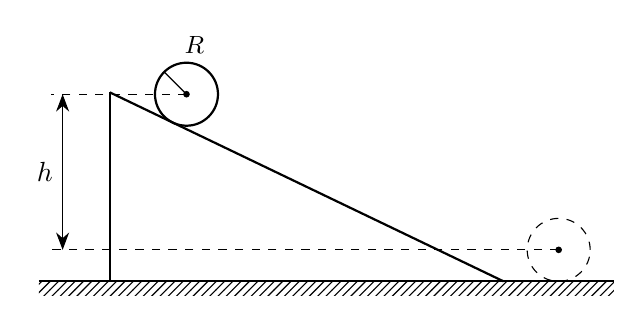
\begin{tikzpicture}[scale=1.0]
  \fill[pattern=north east lines] (-0.9,-0.18) rectangle (6.4,0);
  \draw[thick] (-0.9,0) -- (6.4,0);
  \draw[thick] (0,2.4) -- (0,0);
  \draw[thick] (0,2.4) -- (5.0,0);
  % normal unitaria al plano: (2.4, 5)/5.546
  \coordinate (A) at ({0.8 + 0.4*2.4/5.546},{2.4 - 0.48*0.8 + 0.4*5/5.546});
  \draw[thick] (A) circle (0.4);
  \fill (A) circle (1.2pt);
  \draw[thin] (A) -- ++(135:0.4);
  \node[font=\small] at ($(A)+(0.1,0.62)$) {$R$};
  \coordinate (B) at (5.7,0.4);
  \draw[dashed] (B) circle (0.4);
  \fill (B) circle (1.2pt);
  \draw[dashed, thin] (A) -- (-0.75,{2.4 - 0.48*0.8 + 0.4*5/5.546});
  \draw[dashed, thin] (B) -- (-0.75,0.4);
  \draw[<->] (-0.6,0.4) -- node[left]{$h$} (-0.6,{2.4 - 0.48*0.8 + 0.4*5/5.546});
\end{tikzpicture}
\end{document}
